% Copyright 2004 by Till Tantau <tantau@users.sourceforge.net>.
%
% In principle, this file can be redistributed and/or modified under
% the terms of the GNU Public License, version 2.
%
% However, this file is supposed to be a template to be modified
% for your own needs. For this reason, if you use this file as a
% template and not specifically distribute it as part of a another
% package/program, I grant the extra permission to freely copy and
% modify this file as you see fit and even to delete this copyright
% notice. 

\documentclass{beamer}

% There are many different themes available for Beamer. A comprehensive
% list with examples is given here:
% http://deic.uab.es/~iblanes/beamer_gallery/index_by_theme.html
% You can uncomment the themes below if you would like to use a different
% one:
%\usetheme{AnnArbor}
%\usetheme{Antibes}
%\usetheme{Bergen}
%\usetheme{Berkeley}
%\usetheme{Berlin}
%\usetheme{Boadilla}
%\usetheme{boxes}
%\usetheme{CambridgeUS}
%\usetheme{Copenhagen}
%\usetheme{Darmstadt}
%\usetheme{default}
%\usetheme{Frankfurt}
%\usetheme{Goettingen}
%\usetheme{Hannover}
%\usetheme{Ilmenau}
%\usetheme{JuanLesPins}
%\usetheme{Luebeck}
\usetheme{Madrid}
\usecolortheme{beaver}
%\usetheme{Malmoe}
%\usetheme{Marburg}
%\usetheme{Montpellier}
%\usetheme{PaloAlto}
%\usetheme{Pittsburgh}
%\usetheme{Rochester}
%\usetheme{Singapore}
%\usetheme{Szeged}
%\usetheme{Warsaw}
\usepackage{colortbl}
\graphicspath{ {img/} }

% For algorithms
\usepackage{algorithm}
\usepackage{algorithmic}

% For mathematics
\usepackage{amsmath}
\usepackage{amsfonts}
\usepackage{amssymb}

\title{Parallel Gradient Descent for Multilayer Feedforward Neural Networks}

% A subtitle is optional and this may be deleted
\author[]{Palash Goyal\inst{1}
\and Nitin Kamra\inst{1} \and
        Sungyong Seo\inst{1} \and Vasileios Zois\inst{1}}
% - Give the names in the same order as the appear in the paper.
% - Use the \inst{?} command only if the authors have different
%   affiliation.

%\logo{\includegraphics[height=0.8cm]{target.jpg}\vspace{225pt}}

\institute[University of Southern California] % (optional, but mostly needed)
{
  \inst{1}%
  Department of Computer Science\\
  University of Southern California
 }
% - Use the \inst command only if there are several affiliations.
% - Keep it simple, no one is interested in your street address.

%\date{Conference Name, 2013}
% - Either use conference name or its abbreviation.
% - Not really informative to the audience, more for people (including
%   yourself) who are reading the slides online

%\subject{Theoretical Computer Science}
% This is only inserted into the PDF information catalog. Can be left
% out. 

% If you have a file called "university-logo-filename.xxx", where xxx
% is a graphic format that can be processed by latex or pdflatex,
% resp., then you can add a logo as follows:

% \pgfdeclareimage[height=0.5cm]{university-logo}{university-logo-filename}
% \logo{\pgfuseimage{university-logo}}

% Delete this, if you do not want the table of contents to pop up at
% the beginning of each subsection:
\AtBeginSubsection[]
{
  \begin{frame}<beamer>{Outline}
    \tableofcontents[currentsection,currentsubsection]
  \end{frame}
}

% Let's get started
\begin{document}

\begin{frame}
  \titlepage
\end{frame}

\begin{frame}{Outline}
  \tableofcontents
  % You might wish to add the option [pausesections]
\end{frame}

% Section and subsections will appear in the presentation overview
% and table of contents.

  \section{Introduction}
\label{Intro}

Artificial neural networks are powerful machine learning tools used in many applications including but not limited to search engines, spam and fraud detection, image classification, diagnostic medicine applications and stock market prediction.

Prior to application, neural networks undergo a training phase which is known to be very computationally intensive. This is primarily because the prevailing neural network architectures are implemented using several hidden layers, with each one consisting of thousands to millions of neurons in order to generalize well on diverse inputs. In this case, the resulting number of parameters that need to be trained are in the order of millions.

Furthermore, achieving high accuracy requires considering a large number of training examples (usually in the order of millions). For this reason training a neural network is both a data and resource intensive operation. This calls for efforts to parallelize the training process on multi-core and while emphasizing at utilizing the maximum available bandwidth.

Currently Minibatch Gradient Descent (henceforth called MGD) is the most commonly used optimization algorithm used to train neural networks in supervised settings. It is implemented in a layerwise-recursive fashion which is termed \textit{backpropagation} in the context of neural networks.

In this paper, we have implemented parallel backpropagation to train Multi Layer Perceptrons (MLPs) for classification tasks.
The rest of the paper is organized as follows: section \ref{ProbDesc} presents a description of supervised learning tasks and neural networks as classifiers. Section \ref{BackProp} describes the conventional serial backpropagation algorithm, and an approach to parallelization using multiple threads. Section \ref{GPUBackProp} describes how to implement backpropagation on a GPU with cuda. Section \ref{Exp} describes our datasets and the experiments we performed on them. Section \ref{Results} presents our results obtained for these implementations and analyzes the speedup obtained for various network architectures and increasing problem sizes. It also presents a comparison with the same algorithms implemented using a state-of-the-art neural network library Theano. Finally, we conclude in section \ref{Future} with a discussion of potential applications and future work for this project.
  
  \section{Gradient Descent}

\begin{frame}<beamer>{Outline}
    \tableofcontents[currentsection,currentsubsection]
\end{frame}

\begin{frame}{Gradient Descent}

	Minimize the Mean-Squared Error loss:
	\begin{align*}
	\mathcal{L}_{MSE} (\theta) = \frac{1}{N}\sum_{i=1}^N ( y^{(i)} - f(x^{(i)}; \theta))^2
	\end{align*}
	
	\textbf{Algorithm: Gradient Descent}
	\begin{enumerate}
	\item Initialize all weights $(\theta)$ randomly with small values close to 0.
	\item Repeat until convergence \{
	\begin{equation*}
	\theta_k := \theta_k - \alpha \frac{\partial \mathcal{L}_{MSE}}{\partial \theta_k} \hspace{16pt} \forall k \in \{1,2,...,K\}
	\end{equation*}
	\}
	\end{enumerate}
	
	Minibatch gradient descent considers a subset of examples

\end{frame}
  
  \section{Forward Propagation and Backpropagation}
\label{FBProp}

\begin{frame}<beamer>{Outline}
    \tableofcontents[currentsection,currentsubsection]
\end{frame}

\begin{frame}{Forward Propagation}

	\begin{figure}[!tbp]
	  \centering
	    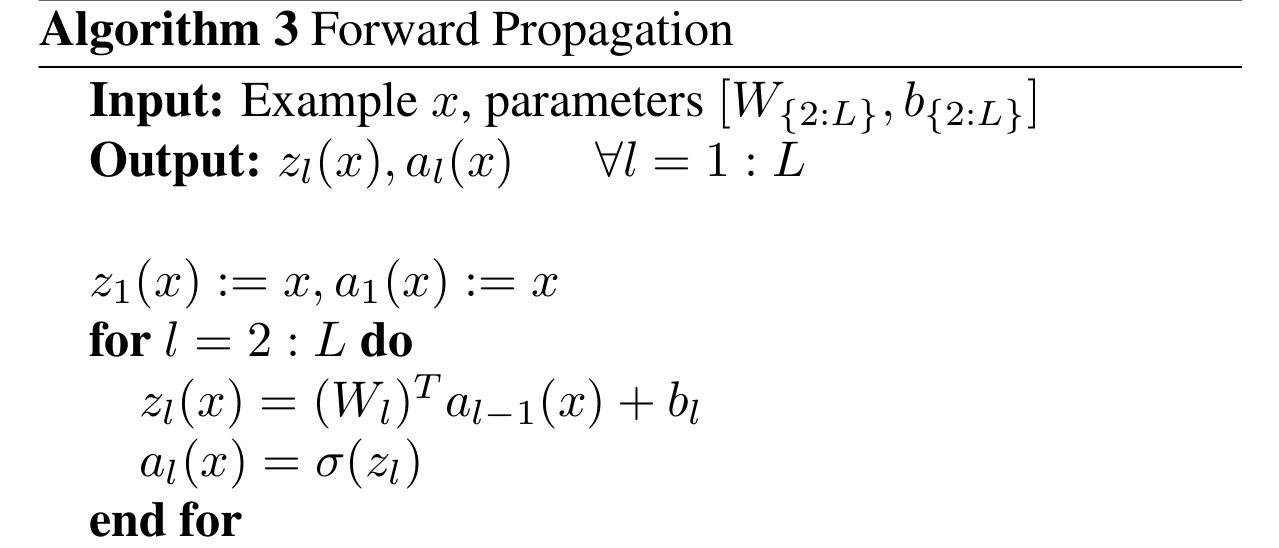
\includegraphics[width=0.8\textwidth]{fwdprop.png}
	\end{figure}

\end{frame}

\begin{frame}{Backpropagation}

	\begin{figure}[!tbp]
	  \centering
	    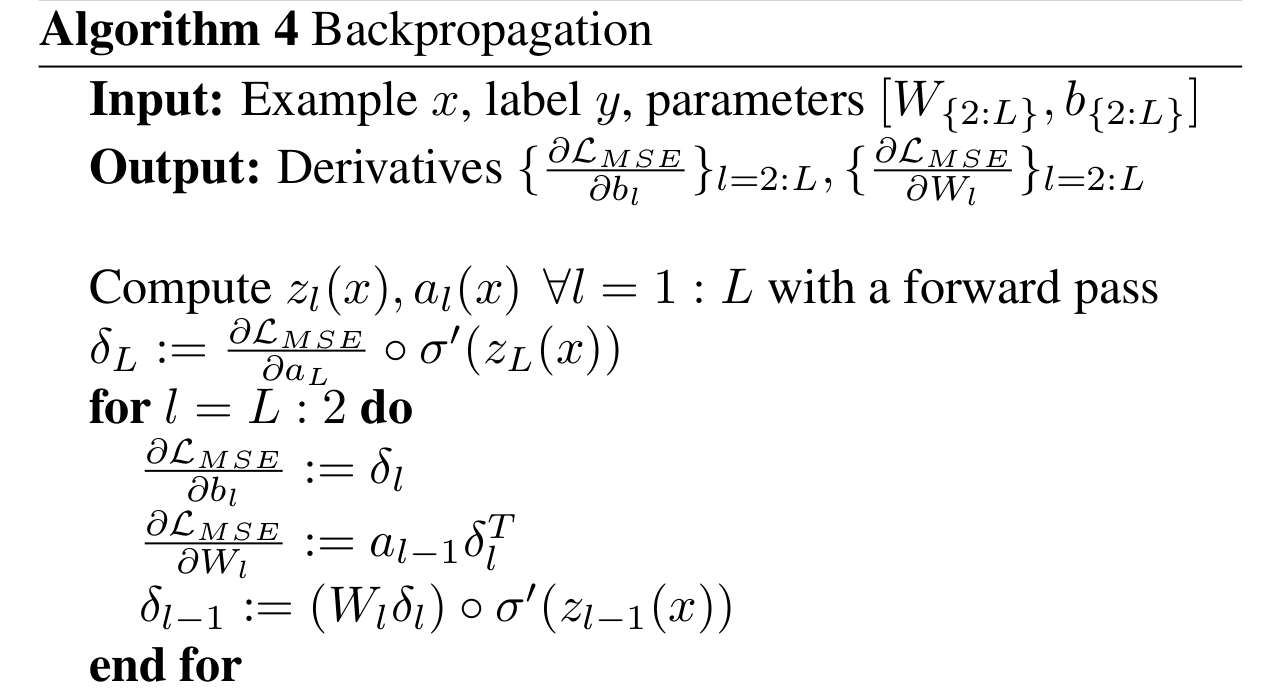
\includegraphics[width=0.8\textwidth]{backprop.png}
	\end{figure}

\end{frame}
  
  \section{Parallel Gradient Descent}
\label{ParGD}

Even with minibatches, the gradient computation can still be a bottleneck for most training algorithms.
There are two potential ways to get rid of this problem and we describe them in the subsequent subsections.

\subsection{Parallel Minibatch Gradient Descent}
\label{sub:PMGD}

Observe that the gradient is a sum of partial gradients with respect to the individual training examples.
So one way to parallelize gradient computation could be by distributing training examples of a minibatch across many processes, letting them compute a partial gradient over their own training examples and then summing up these partial gradients to get the approximate minibatch gradient.
This approach results in a procedure shown in algorithm \ref{alg:PMGD}.
\begin{algorithm}[tb]
   \caption{Parallel Minibatch Gradient Descent}
   \label{alg:PMGD}
\begin{algorithmic}
   \STATE {\bfseries Input:} Dataset $\mathcal{D} = \{x^{(i)},y^{(i)}\}_{i=1:N}$, Step Size $\alpha$, Max Epochs $N_{epoch}$, Batch Size $B$, Num Threads $T$
   \STATE {\bfseries Output:} Parameters $\{\theta_k\}_{k=1:K}$
   \STATE
   \STATE Initialize $\theta$ randomly with small real numbers
   \STATE $ep := 0$
   \REPEAT
   \STATE $ep := ep + 1$
   \STATE Divide $\mathcal{D}$ into batches $\{B_j\}_{j=1:\frac{N}{B}}$ of size $B$ each
   \FOR {$j \in \{1:\frac{N}{B}\}$}
   \STATE Divide $B_j$ into thread-batches $\{B_{jt}\}_{t=1:\frac{B}{T}}$ of size $\frac{B}{T}$
   \STATE \textbf{Thread `t' is forked:}
   \FOR {$k \in \{1:K\}$}
   \STATE $\frac{\partial \mathcal{L}_{MSE}}{\partial \theta_k} \big|_t := \sum_{i \in B_{jt}} ( y^{(i)} - f(x^{(i)}; \theta)) \frac{\partial f(x^{(i)}; \theta)}{\partial \theta_k}$
   \ENDFOR
   \STATE \textbf{Thread `t' joins back 'main'}
   \FOR {$k \in \{1:K\}$}
   \STATE $\frac{\partial \mathcal{L}_{MSE}}{\partial \theta_k} := \frac{1}{B} \sum_t \frac{\partial \mathcal{L}_{MSE}}{\partial \theta_k} \big|_t$
   \ENDFOR
   \STATE $\theta_k := \theta_k - \alpha \frac{\partial \mathcal{L}_{MSE}}{\partial \theta_k} \hspace{16pt} \forall k \in \{1:K\}$
   \ENDFOR
   \UNTIL{$ep \geq N_{epoch}$}
\end{algorithmic}
\end{algorithm}

\subsection{Parallelizing Matrix Computations}

An alternative way to parallelize the gradient computation process can be by parallelizing individual steps of backpropagation (algorithms \ref{alg:FwdPass} and \ref{alg:BackProp}).
Note that the forward propagation and backpropagation algorithms comprise various matrix vector multiplications which can be individually parallelized across multiple threads of execution.
Parallelized matrix-vector multiplications are already efficiently implemented in various linear algebra libraries and we will use the BLAS library to implement this second method of parallelization.

Graphics Processing Units (GPUs) are massively parallel processors that were designed for efficient computer graphics rendering and image processing. In fact, GPUs are very effective when used to execute the graphics rendering pipeline which is a sequence of geometric transformations on small multidimensional vectors. For this reason, GPUs are suitable for executing very fast certain linear algebra operations including but not limited to vector-vector addition, matrix-vector and matrix-matrix multiplication. Moreover, because GPUs consist of many throughput oriented multiprocessors that follow the Single Instruction Multiple Data (SIMD) execution model, they can be very useful for applications that require processing large amount of data.

\begin{figure}[ht]
%\vskip 0.2in
\begin{center}
\centerline{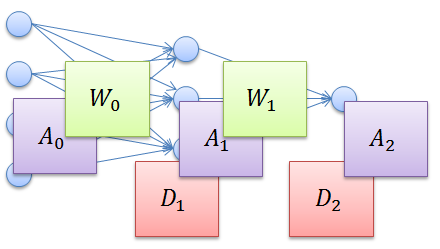
\includegraphics[width=\columnwidth]{gpu_neural_net_data}}
\caption{Abstract layered neural network architecture}
\label{fig:nn_architecture}
\end{center}
\vskip -0.2in
\end{figure}

Training neural networks is a process that can be realized through a series of matrix-matrix multiplications and additions which are applied for a large number of training examples. Every neural network can be defined and operated on by following this abstraction. Back propagation can be implemented as a series of kernel executions that are combined to ultimately compute the change in the weight values caused by the corresponding training batch. In our implementation, a neural network is viewed as a collection of layers, each one consisting of 3 distinct matrices. These matrices store the outgoing weight values $W_i$, the incoming activation values $A_i$ and the delta error values $D_i$ computed by back propagation. The activation values of the input layer (i.e. $A_0$) are the actual training examples in the corresponding batch. The activation values and the delta error values are stored in column-major order. In contrast the weights for each layer are stored in row-major order. The bias values are embedded in the last column of the weight matrix.

\begin{figure}[ht]
%\vskip 0.2in
\begin{center}
\centerline{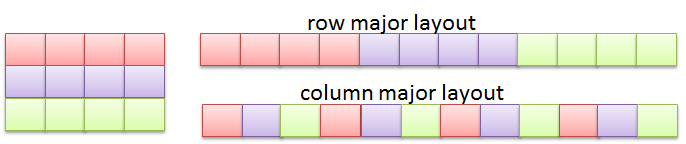
\includegraphics[width=\columnwidth]{gpu_data_layout}}
\caption{Matrix data layout}
\label{fig:data_layout}
\end{center}
\vskip -0.2in
\end{figure}

We decompose back-propagation into 5 steps each one implemented by distinct kernel. The first step, handles the feed forward activation by implementing a tiled matrix-matrix multiplication based on Eq.~\ref{act_kernel}. Here we denote with $f$ the preferred activation function which is usually the sigmoid function. Our implementation is designed around templates and supports user defined activation functions. The feed-forward step is implemented using the tiled matrix-matrix multiplication as it is described in CUDA samples. All threads participate in loading the tiles of the input matrices into shared memory. The threads use registers to accumulate partial results. After parsing the complete matrix each thread applies the activation function on the resulting value before storing it into global memory. All read and write operations to global memory are coalesced and there are no bank conflicts because thread iterate over the secondary matrix dimension in each case. An additional step is required to initialize the thread registers with the bias values.

\begin{equation}\label{act_kernel}
A_{i+1} = f\left(W_{i} \cdot A_{i} + b_i\right), \forall i \in \left[1,L-1\right]
\end{equation}

\begin{equation}\delta_output_kernel
D_{L} = Y - A_{L}
\end{equation}

\begin{equation}\label{delta_kernel}
D_{i} = W_{i}^T \cdot D_{i} \circ d(W_{i-1} \cdot A_{i+1})
\end{equation}

\begin{equation}\label{update_kernel}
W_{i} = W_{i} + \frac{n}{b} \cdot \sum_{j=1}^{b} D_{i+1}^{j} \cdot (A_{i}^j)^T
\end{equation}

Following this previous step, the delta error values are computed for each layer using Eq.~\ref{delta_kernel}. This equation is computed using 3 kernels, one for computing the output layer delta and two more that compute the transpose matrix-matrix multiplication and the hadamard product of the derivative for the corresponding activation function. A variation of the tiled matrix-matrix multiplication kernel is used to perform these operations. For the first kernel, the indexing is changed to enable multiplication with the transpose of the weight matrix. Here accesses to global memory remain coalesced since we order the thread blocks vertically on the weight matrix. However, we incur few bank conflicts when accessing the data in column-major order from shared-memory . In the second case, we chose to re-compute the product of $W_i \cdot A_i$ and multiply it with the result from the previous operation. This is because are goal was to support arbitrary defined activation functions. In case the sigmoid function is used, the derivative can be replaced with $A_i \cdot \left(1.0 - A_i\right)$ which enables significant reduction of the required computation.

Finally, we use the computed activation and the next layer delta matrices (Eq.~\ref{update_kernel}) to update the weights of the corresponding layer depending on the chosen learning rate and batch size. This operation can be considered as another variation of matrix-matrix multiplication where each column from $ D_{i+1}$ and $A_{i}$ are  multiplied to produced a single matrix. The number of resulting matrices are equal to the batch size and are accumulated in thread registers. The resulting summation is multiplied by $\frac{n}{b}$ and added to the weight values of the corresponding layer. For this operation, access to global memory is again coalesced. However, shared memory access incurs many bank conflicts which are proportional to the batch size. In order to improve the performance, the corresponding tiles are loaded transposed into shared memory. This incurs only a single bank conflict during loading and avoids many bank conflicts during the multiplication phase.

  \section{Experimental setup}
\label{Exp}
In this section, we first describe the datasets used for our experiments and the corresponding classification tasks. We then delineate the networks used for each of these datasets and the procedure to determine the values of hyperparameters. This is followed by a description of the evaluation metric of the speedup. All the algorithms were implemented in C++. The reported results were obtained on a Ubuntu 14.04.4 LTS system with 32 cores, 128 GB RAM and a clock speed of 2.6 GHz.  

\subsection{Dataset description}
\label{sub:data_desc}
We test the speedups achieved by the parallel implementation on two public datasets - MNIST and KDD Cup 1999. These datasets have been widely used by the machine learning community to compare different learning algorithms. Their description is as follows:

\begin{itemize}
\item \textbf{MNIST} - This is an image database of handwritten digits which is commonly used for training various image processing systems (Figure \ref{fig:mnist}). The task here is to classify the digit in the image. This dataset was derived from NIST's datasets and was formed by mixing the samples from NIST. This mixing was done because the training and testing datasets in the original NIST dataset were obtained from two different groups of people (Census Bureau employees and high school students). This dataset consists of 60,000 training images and 10,000 testing images, each of size 28$\times$ 28. In our experiments, we further divided the training set into training and validation in 5:1 ratio in order to determine suitable values for the hyperparameters.

\begin{figure}
  \centering
       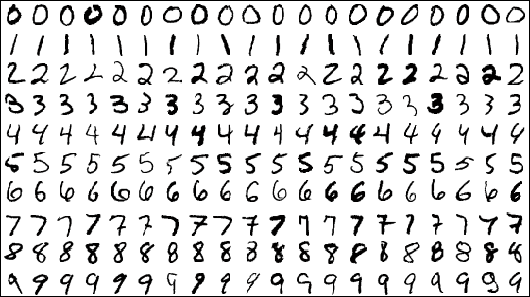
\includegraphics[scale=0.43]{mnist.png}
  \caption{MNIST dataset}
  \label{fig:mnist}
\end{figure}

\item \textbf{KDD Cup 1999} -  This is a dataset which first appeared in the KDD Cup held in 1999. The dataset has about 4 million data points each of which has 42 features. The features are of two types - categorical and integer. The task in the competition was to build a network intrusion detector which can be used to distinguish between good and bad network connections. 
\end{itemize}

\subsection{Network details}
\label{sub:net_det}
We now describe the details of the structure of neural networks used. For our experiments, we use two different configurations of neural network - 
\begin{itemize}
\item \textbf{Net-1h} - This network consists of 3 layers - input layer, one hidden layer and output layer. The input layer has 784 neurons for MNIST dataset and 42 neurons for KDD Cup 1999. The hidden layer is composed of 1024 neurons and the output layer has 10 neurons when used for MNIST dataset and 1 output for KDD Cup 1999.
\item \textbf{Net-2h} - This network is composed of 4 layers - input layer, two hidden layers and output layer. The input and output layer are same as Net-1h and each of the hidden layers has 1024 neurons.
\end{itemize}

\subsection{Hyperparameter selection}
\label{sub:hyper_sel}
Hyperparameter selection, also known as model selection, is an important problem in machine learning. It refers to choosing the optimal hyperparameters for a learning algorithm. It is crucial to select the values for hyperparameters which generalize well. This enables the algorithm to perform well on test data.

In the context of neural networks, hyperparameters refer to learning rate and regularization constant. Since our implementation is free of regularization, we only have one hyperparameter - learning rate. To choose an optimal learning rate, we used the technique of grid search. As mentioned above, we divide the training set into training and validation. We use different learning rates defined in a grid and test the accuracy on the validation data. The rate which gives the highest accuracy on validation is chosen and used to evaluate the performance of the algorithm on test data.

\subsection{Evaluation methodology}
\label{sub:eval}
As has been previously mentioned, this work aims to speed up the learning of neural network by parallelizing backpropagation and running it on GPU. To evaluate our approach and quantify the usefulness of parallelization, we use speed up as our primary measure. We calculate this with respect to the serial implementation on the same network configuration. Speed up may sometimes be misleading and does not capture the efficiency of serial implementation. To resolve this we use another measure - GFLOPS (Billion Floating Point Operations Per Second). This measure is independent of serial implementation and can be used to supplement the speedup metric.

\subsection{Experiments}
\label{sub:exp}
In this paper, we implement the gradient descent algorithm for training neural network. The implementation is 3-fold - serial, parallelization with Pthreads and parallelization with CUDA. The implementation follows from section \ref{BackProp} and section \ref{GPUBackProp}. Please refer to these sections for a detailed explanation of the methods.



  
  \section{Results and Analysis}
\label{Results}

%Provide experiment results: serial \\
%Compare serial vs pthreads vs cuda vs theano. \\
%Provide graphs for speedup with increasing problem size \\
%Analyze speedup with number of threads/cores used \\
%Analyze the level of parallelization obtained \\
%Analyze performance bottlenecks \\
%Do overall analysis and compare obtained results with your expectations\\

As described in previous sections, we compare our implementations with state of the art deep learning library, Theano, in three different parallelizations (Serial/Pthreads/Cuda-C). All experiments are done under the same network structures with MNIST datasets and the number of threads is fixed as 32.

\begin{figure}[ht]
%\vskip 0.2in
\begin{center}
\centerline{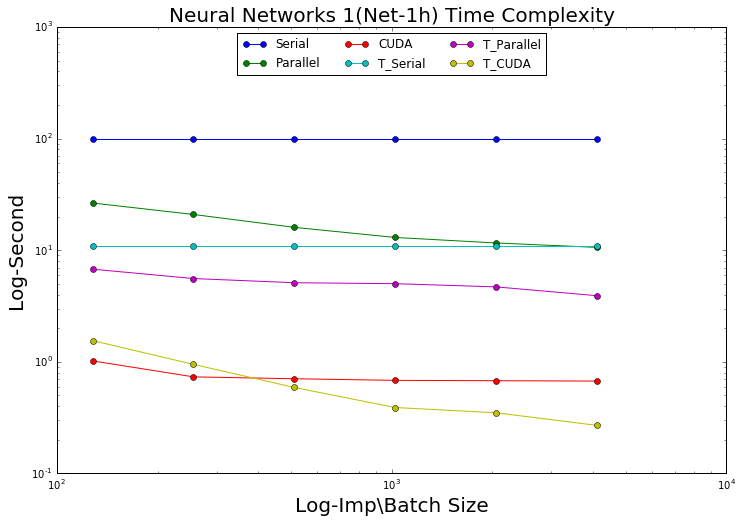
\includegraphics[width=\columnwidth]{../../slide/nn1_time.png}}
\caption{Learning time for Net-1h}
\label{fig:nn1_time}
\end{center}
\vskip -0.4in
\end{figure}

Figure \ref{fig:nn1_time} clearly shows distinct characteristics between serial and parallel computation as well as CPU and GPU based computation. First, the training time for 1 epoch of the serial implementation (Blue curve and Light blue curve) is almost constant over the varying mini batch size. It is obvious result because regardless of the size of each mini batch training data is accessed sequentially. On the other hand, the parallel learning time (Green curve) shows decreased training time due to multithreads distribution as we expected. One thing we should note is that the parallelism is enhanced when larger size of batch is used because the number of allocations of data into each thread is reduced. When smaller batch size is used, we need to assign each data into the corresponding thread more frequently and it causes more overheads. Moreover, as the last step, we need to combine all the results from every threads (which is called the reduction process) and the number of the reduction processes is also increased for smaller batch size. This behavior is shown commonly in the parallel computation based on Theano (T-Parallel).\\
In case of GPU based computation, the overall performance is significantly improved because GPU usually have much more cores which are specialized for repetitive operations such as matrix multiplications than CPU. As a result, GPU provides much faster learning time than that of CPU in general due to less number of allocation/reduction processes.\\
The faster computation by the parallelization is able to be captured by calculating GFLOPS. Figure \ref{fig:nn1_gflops} shows that parallelization provide much larger number of floating point operations than serial, thus, single thread computation.
\begin{figure}[ht]
%\vskip 0.2in
\begin{center}
\centerline{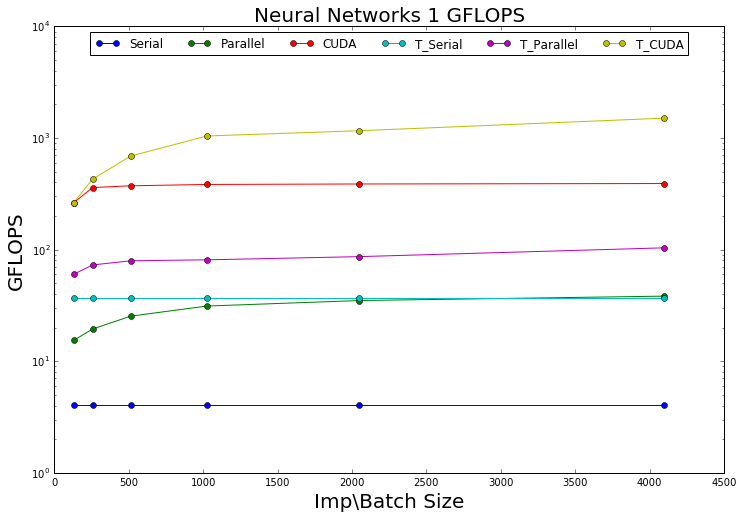
\includegraphics[width=\columnwidth]{../../slide/nn1_gflops.png}}
\caption{GFLOPS for Net-1h}
\label{fig:nn1_gflops}
\end{center}
\vskip -0.4in
\end{figure}

\textbf{BLAS} As Basic Linear Algebra Subprograms, BLAS has been crucial workhorse in heavy numerical computing. By replacing the self-built matrix-vector product libraries with BLAS functions, we could obtain hugely improved results (even faster than Theano). Note that the execution time of BLAS doesn't depend on the number of threads because it parallelizes each Matrix-vector product and hence each thread executes different parts of the same example. The serial implementation is still a bit slower than Theano but is faster than our previous implementation by about 10 times. This way shows that the optimized parallelism gives speed-up over Naive serial implementation. \\

\textbf{Bottleneck} In ideal case, by increasing the size of the batch, the number of overheads (allocation/reduction) is exponentially decreased. However, our experiment results show that there are some performance bottlenecks. In our implementation, shared memory bank conflicts which reduce the parallelism when threads access the shared memory appear when the number of batch increases. When the dimensions (i.e.number of neurons between layers) of the neural network is not perfect multiple of 32 then some threads do not participate in the computation so they are doing no work but still have to wait on the barrier. As a result, it causes degraded parallelism.\\

Overall, we demonstrate that the parallel computation is significantly faster than the serial computation by utilizing multithreads based on the mini batch in the multicore machine. Moreover, by dividing training datasets into larger mini batches, we are able to better performance than that of smaller batch size due to reduced overheads. Similarly, the training time and GFLOPS are improved in the second networks (Net-2h) (See Figure \ref{fig:nn2_time},\ref{fig:nn2_gflops}). 
\begin{figure}[ht]
%\vskip 0.2in
\begin{center}
\centerline{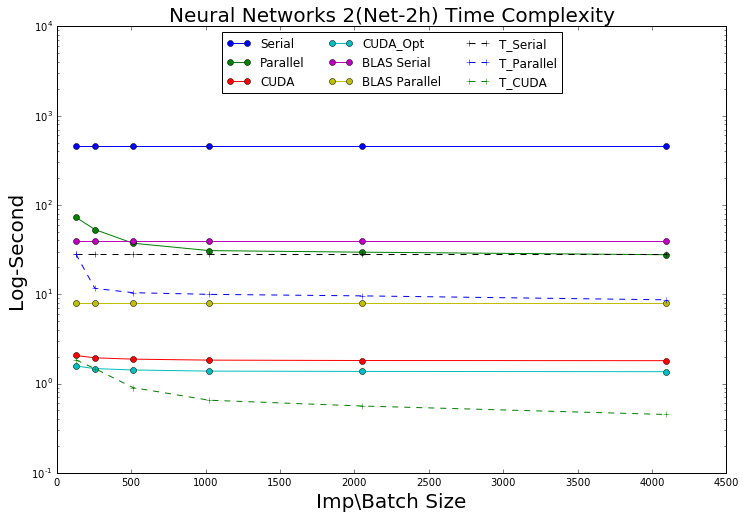
\includegraphics[width=\columnwidth]{../../slide/nn2_time.png}}
\caption{Learning time for Net-2h}
\label{fig:nn2_time}
\end{center}
\vskip -0.4in
\end{figure}
\begin{figure}[ht]
\vskip 0.2in
\begin{center}
\centerline{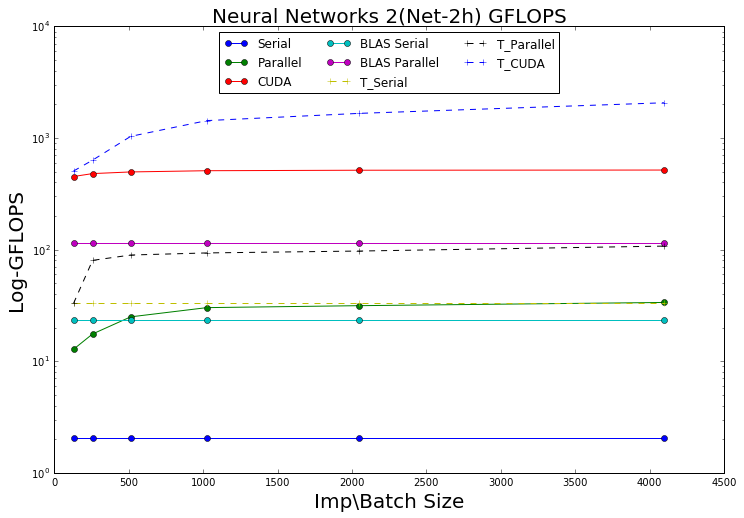
\includegraphics[width=\columnwidth]{../../slide/nn2_gflops.png}}
\caption{GFLOPS for Net-2h}
\label{fig:nn2_gflops}
\end{center}
\vskip -0.4in
\end{figure}





\end{document}